\chapter{The design of the sensor network}
% This chapter describes the design of the sensor network.

\section{Block diagram}
\subsection{Node}
The node as an any device that transmits data in the network. In the star network topology it could be only a sensor or an actuator accessed by the gateway, because there are no routing devices or other. \cite{wsn01}.
\subsection{Gateway}
The gateway handles the communication with all the nodes and transmits the data to other network or device \cite{wsn01}. 
In this case the gateway is accessed by the LAN through RS-485 interface. 
\begin{figure}[!h]
    \centering
    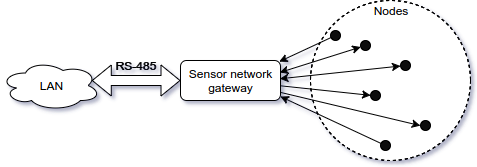
\includegraphics[width=1\textwidth]{LPwSN_bd}
    \caption{The block diagram of the sensor network}
    \label{fig:Typical structure of a card}
\end{figure}


\section{The requirements for the wireless technology}
The main requirement for the designed network is ability to add many various nodes which are available at the market to the network, so we don't have to make our own nodes for every kind of application.
The other requirements are price, power consumption, range etc.


\section{The final choose of the low power wireless technology}
From all the compared technologies in the table in appendix is chosen LoRa, because its nodes are easy to implement to the network with no restrictions. For example there is also many BLE nodes available at the market, but many of manufacturers say that their nodes are compatible only with their own network gateway so it may not be possible to add the node to our designed network. 
To make it simple and cheap only single channel gateway is used which means that all the devices in the network must be configured to one predefined channel and SF. 
